\documentclass{article}
\usepackage[top=0.5in, bottom=0.5in, left=1.25in, right=1.25in]{geometry}

\usepackage{amsmath, array, enumerate, sfmath, pgfplots, pgfplotstable, tcolorbox, graphicx, color, colortbl, multicol}
\pgfplotsset{compat = newest}
\usepgfplotslibrary{statistics}
\usetikzlibrary{arrows.meta}
\renewcommand{\familydefault}{\sfdefault}
\raggedright
\pagestyle{empty}

\newcounter{example}[section]
\newenvironment{example}[1][]{\refstepcounter{example}\par\medskip
   {\color{red}\textbf{Example~\theexample. #1}}}{\medskip}

\begin{document}

\section*{Linear Regression}

\begin{tcolorbox}[colframe=orange!70!white, coltitle=black, title=\textbf{Summary}]
\begin{enumerate}
    \item Regression is all about prediction.
    \item We can calculate the strength of an association (the \textit{correlation}) between two variables.
    \item ``Fundamental Theorem of Statistics": \textbf{Prediction = Reality + Error}
\end{enumerate}
\end{tcolorbox}
\vspace{0.75in}

\begin{tcolorbox}[colframe=green!20!black, colback = green!30!white,title=\textbf{Linear Correlation Coefficient}]
The \textbf{linear correlation coefficient}, $r$, is a numerical value with $-1 \leq r \leq 1$ that measures the type of linear correlation of a bivariate data set.
\end{tcolorbox}
\vspace{0.5in}

\begin{itemize}
	\item $r > 0$: positive linear correlation
	\item $r = 0$: no linear correlation
	\item $r < 0$: negative linear correlation
\end{itemize}
\vspace{0.5in}

\[r = \frac{\sum (x-\overline{x})(y-\overline{y})}{\sqrt{\sum(x-\overline{x})^2 \cdot \sum(y-\overline{y})^2}}\]	
\vspace{0.5in}

\begin{itemize}
    \item Closer $r$ is to 1 (or $-1$) $\longrightarrow$ the more the data points ``fall in line."
    \item Closer $r$ is to 0 $\longrightarrow$ the more the data points resemble a ``cloud"
\end{itemize}

\vfill 

\begin{center}
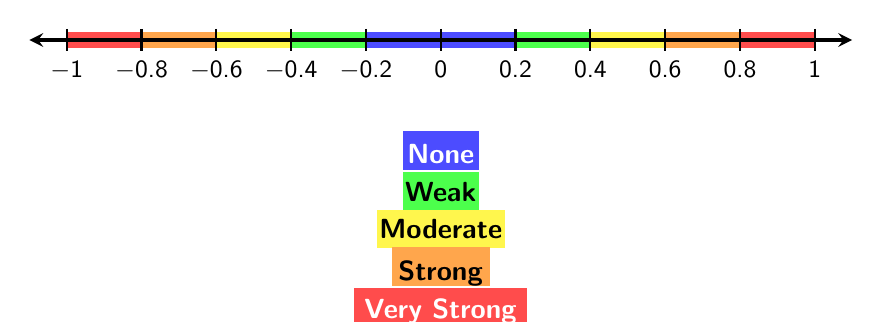
\begin{tikzpicture}[scale=0.95]
\draw [color=red!70, fill=red!70] (-5,-0.1) rectangle (5,0.1);
\draw [color=orange!70, fill=orange!70] (-4,-0.1) rectangle (4,0.1);
\draw [color=yellow!70, fill=yellow!70] (-3,-0.1) rectangle (3,0.1);
\draw [color=green!70, fill=green!70] (-2,-0.1) rectangle (2,0.1);
\draw [color=blue!70, fill=blue!70] (-1,-0.1) rectangle (1,0.1);
\draw [<->, >=stealth, very thick] (-5.5,0) -- (5.5,0);
\foreach \x in {-5,-4,...,5}
\draw [thick] (\x, 0.15) -- (\x,-0.15);
\node at (-5,-0.15) [below] {\small $-1$};
\node at (-4,-0.15) [below] {\small $-0.8$};
\node at (-3,-0.15) [below] {\small $-0.6$};
\node at (-2,-0.15) [below] {\small $-0.4$};
\node at (-1,-0.15) [below] {\small $-0.2$};
\node at (0,-0.15) [below] {\small $0$};
\node at (1,-0.15) [below] {\small $0.2$};
\node at (2,-0.15) [below] {\small $0.4$};
\node at (3,-0.15) [below] {\small $0.6$};
\node at (4,-0.15) [below] {\small $0.8$};
\node at (5,-0.15) [below] {\small $1$};
\raisebox{-0.5cm}{
\draw [color=blue!70, fill=blue!70] (-0.5,-1.2) rectangle (0.5,-0.7);
\node at (0,-1) {\color{white}\textbf{None}};
\draw [color=green!70, fill=green!70] (-0.5,-1.75) rectangle (0.5,-1.25);
\node at (0,-1.5) {\color{black}\textbf{Weak}};
\draw [color=yellow!70, fill=yellow!70] (-0.85,-2.25) rectangle (0.85,-1.75);
\node at (0,-2) {\color{black}\textbf{Moderate}};
\draw [color=orange!70, fill=orange!70] (-0.65,-2.75) rectangle (0.65,-2.25);
\node at (0,-2.6) {\color{black}\textbf{Strong}};
\draw [color=red!70, fill=red!70] (-1.15,-3.35) rectangle (1.15,-2.8);
\node at (0,-3.1) {\color{white}\textbf{Very Strong}}; }
\end{tikzpicture}
\vspace{12pt}

\emph{Note}: These interpretations are not universal.
\end{center}

\vfill
\newpage 

\begin{example}
Find and interpret the linear correlation coefficient. \newline\\
\begin{tabular}{c|c}
$x$ & $y$ \\ \hline
7.6 & 19.1 \\
9.2 & 22.9 \\
3.3 & 10.3 \\
1.1 & 6.6 \\
3.7 & 10.6 \\
3.9 & 11.3 \\
4.6 & 12.9 \\
2.3 & 8.6 \\
5.1 & 15.2 \\
5.3 & 15.1 \\
2.5 & 13 \\
3.4 & 11.2 \\
3.1 & 10.6 \\
1.7 & 6.8 \\
3.7 & 13.7 \\
\end{tabular}
\end{example}

\vfill 

% \begin{tabular}{c|c|c|c|c|c|c|c|c|c|c|c|c|c|c|c}
%     $x$ & 7.6 & 9.2 & 3.3 & 1.1 & 3.7 & 3.9 & 4.6 & 2.3 & 5.1 & 5.3 & 2.5 & 3.4 & 3.1 & 1.7 & 3.7 \\ \hline 
%     $y$ & 19.1 & 22.9 & 10.3 & 6.6 & 10.6 & 11.3 & 12.9 & 8.6 & 15.2 & 15.1 & 13 & 11.2 & 10.6 & 6.8 & 13.7 \\
% \end{tabular}

Given our data set, we also want to be able to predict values.

To do this, we can create the {\color{blue}\textbf{least squares regression equation}}, (also called the \emph{line of best fit})\\
Which {\color{red}\textbf{minimizes}} the total squared distance each data point is from the prediction line:

\[\hat{y} = mx + b\]

\vfill 

\begin{center}
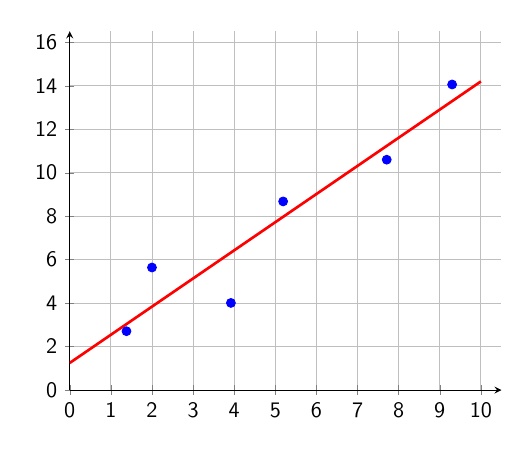
\begin{tikzpicture}[scale=0.8]
\begin{axis}[
	axis lines = left, grid,
	xmin = 0, xmax = 10.5, ymin = 0, ymax = 16.5,
	xtick = {0,1,...,10}, ytick = {0,2,...,16}
]
\addplot[color=blue, only marks] coordinates {
(9.3,14.06)
(5.19,8.68)
(2,5.64)
(7.71,10.6)
(1.38,2.71)
(3.92,4.01)
};
\addplot [color=red, domain=0:10, very thick] {1.295*x + 1.25};
\end{axis}
\end{tikzpicture}
\end{center}

\vspace{1in}

\[m = r\left(\frac{\sigma_y}{\sigma_x}\right)   \quad \text{and} \quad 
b = \overline{y} - m\left(\overline{x}\right)\]

\vfill 
\newpage 

\begin{example}
Find the least squares regression equation for the data set from Example 1. Round your parameters to 3 decimal places.
% \begin{tabular}{c|c}
% $x$ & $y$ \\ \hline
% 7.6 & 19.1 \\
% 9.2 & 22.9 \\
% 3.3 & 10.3 \\
% 1.1 & 6.6 \\
% 3.7 & 10.6 \\
% 3.9 & 11.3 \\
% 4.6 & 12.9 \\
% 2.3 & 8.6 \\
% 5.1 & 15.2 \\
% 5.3 & 15.1 \\
% 2.5 & 13 \\
% 3.4 & 11.2 \\
% 3.1 & 10.6 \\
% 1.7 & 6.8 \\
% 3.7 & 13.7 
% \end{tabular}
\end{example}

\vspace{1.75in}


\begin{example}
Use the regression equation from the previous example to predict the values of the response variable for each given explanatory variable.
\begin{multicols}{2}
\begin{enumerate}[(a)]
    \item $x = 6$
    \item $x = 11$
\end{enumerate}
\end{multicols}
\end{example}

\vspace{1.75in}

\subsection*{Residual Error}

Suppose we obtain an actual data point when $x = 6$ and observe that $y = 16$. 
\vspace{0.25in}

\[
\text{Residual } (\epsilon) = \text{observed value} - \text{expected value}
\]

\vspace{2in}

We could then add the point $(6, 16)$ to our data set to get a more-accurate prediction equation.

\newpage 

\subsection*{Coefficient of Determination}

The value $r^2$ is called the {\color{blue}\textbf{coefficient of determination}} 
\begin{itemize}
    \item Tells what percentage of the variability in the response ($y$) variable is due to the relationship between $x$ and $y$.
    \item The rest may be due to such things as lurking variables or confounding. 
    \item Since $-1 \leq r \leq 1 \longrightarrow 0 \leq r^2 \leq 1$
    \vspace{0.5in}
    \item But what does $r^2$ \emph{actually} do???
    \begin{itemize}
        \item Without our regression equation, the best predictor for response variables ($y$ values) would be the average of the $y$-coordinates, $\overline{y}$. \newline\\
        \item The value of $r^2$ represents \textbf{how much of a decrease in prediction error we get} from using our regression equation rather than $\overline{y}$. \newline\\
        \item If $r$ (and hence $r^2$) is close to 0, then the linear regression equation is not going to be a good predictor. So you could just use $\overline{y}$.
    \end{itemize}
\end{itemize}
\vspace{1.5in}

\begin{example}
Interpret the value of $r^2$ from example 1.
\end{example}
\end{document}
